\documentclass[11pt,compress,t,notes=noshow, aspectratio=169, xcolor=table]{beamer}

\usepackage{../../style/lmu-lecture}
\usepackage{siunitx}
% Defines macros and environments
\usepackage[]{graphicx}
\usepackage[]{color}
% maxwidth is the original width if it is less than linewidth
% otherwise use linewidth (to make sure the graphics do not exceed the margin)
\makeatletter
\def\maxwidth{ %
\ifdim\Gin@nat@width>\linewidth
\linewidth
\else
\Gin@nat@width
\fi
}
\makeatother
%\usepackage[fontsize=10.5pt]{scrextend}
\definecolor{ggred}{rgb}{0.973, 0.463, 0.427}
\definecolor{ggblue}{rgb}{0, 0.749, 0.769}
\definecolor{fgcolor}{rgb}{0.345, 0.345, 0.345}
\newcommand{\hlnum}[1]{\textcolor[rgb]{0.686,0.059,0.569}{#1}}%
\newcommand{\hlstr}[1]{\textcolor[rgb]{0.192,0.494,0.8}{#1}}%
\newcommand{\hlcom}[1]{\textcolor[rgb]{0.678,0.584,0.686}{\textit{#1}}}%
\newcommand{\hlopt}[1]{\textcolor[rgb]{0,0,0}{#1}}%
\newcommand{\hlstd}[1]{\textcolor[rgb]{0.345,0.345,0.345}{#1}}%
\newcommand{\hlkwa}[1]{\textcolor[rgb]{0.161,0.373,0.58}{\textbf{#1}}}%
\newcommand{\hlkwb}[1]{\textcolor[rgb]{0.69,0.353,0.396}{#1}}%
\newcommand{\hlkwc}[1]{\textcolor[rgb]{0.333,0.667,0.333}{#1}}%
\newcommand{\hlkwd}[1]{\textcolor[rgb]{0.737,0.353,0.396}{\textbf{#1}}}%
\newcommand{\predvar}{Var\left[\hat{f}(\xv)\right]}
\let\hlipl\hlkwb

\usepackage{pdfpages}
\usepackage{framed}
\makeatletter
\newenvironment{kframe}{%
\def\at@end@of@kframe{}%
\ifinner\ifhmode%
\def\at@end@of@kframe{\end{minipage}}%
\begin{minipage}{\columnwidth}%
\fi\fi%
\def\FrameCommand##1{\hskip\@totalleftmargin \hskip-\fboxsep
\colorbox{shadecolor}{##1}\hskip-\fboxsep
% There is no \\@totalrightmargin, so:
\hskip-\linewidth \hskip-\@totalleftmargin \hskip\columnwidth}%
\MakeFramed {\advance\hsize-\width
\@totalleftmargin\z@ \linewidth\hsize
\@setminipage}}%
{\par\unskip\endMakeFramed%
\at@end@of@kframe}
\makeatother

\definecolor{shadecolor}{rgb}{.97, .97, .97}
\definecolor{messagecolor}{rgb}{0, 0, 0}
\definecolor{warningcolor}{rgb}{1, 0, 1}
\definecolor{errorcolor}{rgb}{1, 0, 0}
\newenvironment{knitrout}{}{} % an empty environment to be redefined in TeX

\usepackage{alltt}
\newcommand{\SweaveOpts}[1]{}  % do not interfere with LaTeX
\newcommand{\SweaveInput}[1]{} % because they are not real TeX commands
\newcommand{\Sexpr}[1]{}       % will only be parsed by R

\usepackage[english]{babel}
\usepackage[utf8]{inputenc}

\usepackage[export]{adjustbox}
\usepackage{dsfont}
\usepackage{verbatim}
\usepackage{amsmath}
\usepackage{amsfonts}
\usepackage{bm}
\usepackage{csquotes}
\usepackage{multirow}
\usepackage{longtable}
\usepackage{booktabs}
\usepackage{enumerate}
\usepackage[absolute,overlay]{textpos}
\usepackage{psfrag}
\usepackage{algorithm}
\usepackage{algpseudocode}
\usepackage{eqnarray}
\usepackage{arydshln}
\usepackage{tabularx}
\usepackage{placeins}
\usepackage{tikz}
\usepackage{setspace}
\usepackage{colortbl}
\usepackage{mathtools}
\usepackage{wrapfig}
\usepackage{bm}
\usepackage[backend=biber]{biblatex}

\usetikzlibrary{tikzmark, shapes,arrows,automata,positioning,calc,chains,trees,  shadows, decorations.pathreplacing}
\tikzset{
%Define standard arrow tip
>=stealth',
%Define style for boxes
punkt/.style={
rectangle,
rounded corners,
draw=black, very thick,
text width=6.5em,
minimum height=2em,
text centered},
% Define arrow style
pil/.style={
->,
thick,
shorten <=2pt,
shorten >=2pt,}
}

\usepackage{subfig}

\usepackage{bbm}
%\newcommand\hmmax{0}
%\newcommand\bmmax{0}
% basic latex stuff
\newcommand{\pkg}[1]{{\fontseries{b}\selectfont #1}} %fontstyle for R packages
\newcommand{\lz}{\vspace{0.5cm}} %vertical space
\newcommand{\dlz}{\vspace{1cm}} %double vertical space
\newcommand{\oneliner}[1] % Oneliner for important statements
{\begin{block}{}\begin{center}\begin{Large}#1\end{Large}\end{center}\end{block}}

% Latexmath Notation
% math spaces
\ifdefined\N                                                                
\renewcommand{\N}{\mathds{N}} % N, naturals
\else \newcommand{\N}{\mathds{N}} \fi 
\newcommand{\Z}{\mathds{Z}} % Z, integers
\newcommand{\Q}{\mathds{Q}} % Q, rationals
\newcommand{\R}{\mathds{R}} % R, reals
\ifdefined\C 
  \renewcommand{\C}{\mathds{C}} % C, complex
\else \newcommand{\C}{\mathds{C}} \fi
\newcommand{\continuous}{\mathcal{C}} % C, space of continuous functions
\newcommand{\M}{\mathcal{M}} % machine numbers
\newcommand{\epsm}{\epsilon_m} % maximum error

% counting / finite sets
\newcommand{\setzo}{\{0, 1\}} % set 0, 1
\newcommand{\setmp}{\{-1, +1\}} % set -1, 1
\newcommand{\unitint}{[0, 1]} % unit interval

% basic math stuff
\newcommand{\xt}{\tilde x} % x tilde
\newcommand{\argmax}{\operatorname{arg\,max}} % argmax
\newcommand{\argmin}{\operatorname{arg\,min}} % argmin
\newcommand{\argminlim}{\mathop{\mathrm{arg\,min}}\limits} % argmax with limits
\newcommand{\argmaxlim}{\mathop{\mathrm{arg\,max}}\limits} % argmin with limits  
\newcommand{\sign}{\operatorname{sign}} % sign, signum
\newcommand{\I}{\mathbb{I}} % I, indicator
\newcommand{\order}{\mathcal{O}} % O, order
\newcommand{\pd}[2]{\frac{\partial{#1}}{\partial #2}} % partial derivative
\newcommand{\floorlr}[1]{\left\lfloor #1 \right\rfloor} % floor
\newcommand{\ceillr}[1]{\left\lceil #1 \right\rceil} % ceiling

% sums and products
\newcommand{\sumin}{\sum\limits_{i=1}^n} % summation from i=1 to n
\newcommand{\sumim}{\sum\limits_{i=1}^m} % summation from i=1 to m
\newcommand{\sumjn}{\sum\limits_{j=1}^n} % summation from j=1 to p
\newcommand{\sumjp}{\sum\limits_{j=1}^p} % summation from j=1 to p
\newcommand{\sumik}{\sum\limits_{i=1}^k} % summation from i=1 to k
\newcommand{\sumkg}{\sum\limits_{k=1}^g} % summation from k=1 to g
\newcommand{\sumjg}{\sum\limits_{j=1}^g} % summation from j=1 to g
\newcommand{\meanin}{\frac{1}{n} \sum\limits_{i=1}^n} % mean from i=1 to n
\newcommand{\meanim}{\frac{1}{m} \sum\limits_{i=1}^m} % mean from i=1 to n
\newcommand{\meankg}{\frac{1}{g} \sum\limits_{k=1}^g} % mean from k=1 to g
\newcommand{\prodin}{\prod\limits_{i=1}^n} % product from i=1 to n
\newcommand{\prodkg}{\prod\limits_{k=1}^g} % product from k=1 to g
\newcommand{\prodjp}{\prod\limits_{j=1}^p} % product from j=1 to p

% linear algebra
\newcommand{\one}{\boldsymbol{1}} % 1, unitvector
\newcommand{\zero}{\mathbf{0}} % 0-vector
\newcommand{\id}{\boldsymbol{I}} % I, identity
\newcommand{\diag}{\operatorname{diag}} % diag, diagonal
\newcommand{\trace}{\operatorname{tr}} % tr, trace
\newcommand{\spn}{\operatorname{span}} % span
\newcommand{\scp}[2]{\left\langle #1, #2 \right\rangle} % <.,.>, scalarproduct
\newcommand{\mat}[1]{\begin{pmatrix} #1 \end{pmatrix}} % short pmatrix command
\newcommand{\Amat}{\mathbf{A}} % matrix A
\newcommand{\Deltab}{\mathbf{\Delta}} % error term for vectors

% basic probability + stats
\renewcommand{\P}{\mathds{P}} % P, probability
\newcommand{\E}{\mathds{E}} % E, expectation
\newcommand{\var}{\mathsf{Var}} % Var, variance
\newcommand{\cov}{\mathsf{Cov}} % Cov, covariance
\newcommand{\corr}{\mathsf{Corr}} % Corr, correlation
\newcommand{\normal}{\mathcal{N}} % N of the normal distribution
\newcommand{\iid}{\overset{i.i.d}{\sim}} % dist with i.i.d superscript
\newcommand{\distas}[1]{\overset{#1}{\sim}} % ... is distributed as ...

% machine learning
\newcommand{\Xspace}{\mathcal{X}} % X, input space
\newcommand{\Yspace}{\mathcal{Y}} % Y, output space
\newcommand{\nset}{\{1, \ldots, n\}} % set from 1 to n
\newcommand{\pset}{\{1, \ldots, p\}} % set from 1 to p
\newcommand{\gset}{\{1, \ldots, g\}} % set from 1 to g
\newcommand{\Pxy}{\mathbb{P}_{xy}} % P_xy
\newcommand{\Exy}{\mathbb{E}_{xy}} % E_xy: Expectation over random variables xy
\newcommand{\xv}{\mathbf{x}} % vector x (bold)
\newcommand{\xtil}{\tilde{\mathbf{x}}} % vector x-tilde (bold)
\newcommand{\yv}{\mathbf{y}} % vector y (bold)
\newcommand{\xy}{(\xv, y)} % observation (x, y)
\newcommand{\xvec}{\left(x_1, \ldots, x_p\right)^\top} % (x1, ..., xp) 
\newcommand{\Xmat}{\mathbf{X}} % Design matrix
\newcommand{\allDatasets}{\mathds{D}} % The set of all datasets
\newcommand{\allDatasetsn}{\mathds{D}_n}  % The set of all datasets of size n 
\newcommand{\D}{\mathcal{D}} % D, data
\newcommand{\Dn}{\D_n} % D_n, data of size n
\newcommand{\Dtrain}{\mathcal{D}_{\text{train}}} % D_train, training set
\newcommand{\Dtest}{\mathcal{D}_{\text{test}}} % D_test, test set
\newcommand{\xyi}[1][i]{\left(\xv^{(#1)}, y^{(#1)}\right)} % (x^i, y^i), i-th observation
\newcommand{\Dset}{\left( \xyi[1], \ldots, \xyi[n]\right)} % {(x1,y1)), ..., (xn,yn)}, data
\newcommand{\defAllDatasetsn}{(\Xspace \times \Yspace)^n} % Def. of the set of all datasets of size n 
\newcommand{\defAllDatasets}{\bigcup_{n \in \N}(\Xspace \times \Yspace)^n} % Def. of the set of all datasets 
\newcommand{\xdat}{\left\{ \xv^{(1)}, \ldots, \xv^{(n)}\right\}} % {x1, ..., xn}, input data
\newcommand{\ydat}{\left\{ \yv^{(1)}, \ldots, \yv^{(n)}\right\}} % {y1, ..., yn}, input data
\newcommand{\yvec}{\left(y^{(1)}, \hdots, y^{(n)}\right)^\top} % (y1, ..., yn), vector of outcomes
\renewcommand{\xi}[1][i]{\xv^{(#1)}} % x^i, i-th observed value of x
\newcommand{\yi}[1][i]{y^{(#1)}} % y^i, i-th observed value of y 
\newcommand{\xivec}{\left(x^{(i)}_1, \ldots, x^{(i)}_p\right)^\top} % (x1^i, ..., xp^i), i-th observation vector
\newcommand{\xj}{\xv_j} % x_j, j-th feature
\newcommand{\xjvec}{\left(x^{(1)}_j, \ldots, x^{(n)}_j\right)^\top} % (x^1_j, ..., x^n_j), j-th feature vector
\newcommand{\phiv}{\mathbf{\phi}} % Basis transformation function phi
\newcommand{\phixi}{\mathbf{\phi}^{(i)}} % Basis transformation of xi: phi^i := phi(xi)

%%%%%% ml - models general
\newcommand{\lamv}{\bm{\lambda}} % lambda vector, hyperconfiguration vector
\newcommand{\Lam}{\bm{\Lambda}}	 % Lambda, space of all hpos
% Inducer / Inducing algorithm
\newcommand{\preimageInducer}{\left(\defAllDatasets\right)\times\Lam} % Set of all datasets times the hyperparameter space
\newcommand{\preimageInducerShort}{\allDatasets\times\Lam} % Set of all datasets times the hyperparameter space
% Inducer / Inducing algorithm
\newcommand{\ind}{\mathcal{I}} % Inducer, inducing algorithm, learning algorithm 

% continuous prediction function f
\newcommand{\ftrue}{f_{\text{true}}}  % True underlying function (if a statistical model is assumed)
\newcommand{\ftruex}{\ftrue(\xv)} % True underlying function (if a statistical model is assumed)
\newcommand{\fx}{f(\xv)} % f(x), continuous prediction function
\newcommand{\fdomains}{f: \Xspace \rightarrow \R^g} % f with domain and co-domain
\newcommand{\Hspace}{\mathcal{H}} % hypothesis space where f is from
\newcommand{\fbayes}{f^{\ast}} % Bayes-optimal model
\newcommand{\fxbayes}{f^{\ast}(\xv)} % Bayes-optimal model
\newcommand{\fkx}[1][k]{f_{#1}(\xv)} % f_j(x), discriminant component function
\newcommand{\fh}{\hat{f}} % f hat, estimated prediction function
\newcommand{\fxh}{\fh(\xv)} % fhat(x)
\newcommand{\fxt}{f(\xv ~|~ \thetab)} % f(x | theta)
\newcommand{\fxi}{f\left(\xv^{(i)}\right)} % f(x^(i))
\newcommand{\fxih}{\hat{f}\left(\xv^{(i)}\right)} % f(x^(i))
\newcommand{\fxit}{f\left(\xv^{(i)} ~|~ \thetab\right)} % f(x^(i) | theta)
\newcommand{\fhD}{\fh_{\D}} % fhat_D, estimate of f based on D
\newcommand{\fhDtrain}{\fh_{\Dtrain}} % fhat_Dtrain, estimate of f based on D
\newcommand{\fhDnlam}{\fh_{\Dn, \lamv}} %model learned on Dn with hp lambda
\newcommand{\fhDlam}{\fh_{\D, \lamv}} %model learned on D with hp lambda
\newcommand{\fhDnlams}{\fh_{\Dn, \lamv^\ast}} %model learned on Dn with optimal hp lambda 
\newcommand{\fhDlams}{\fh_{\D, \lamv^\ast}} %model learned on D with optimal hp lambda 

% discrete prediction function h
\newcommand{\hx}{h(\xv)} % h(x), discrete prediction function
\newcommand{\hh}{\hat{h}} % h hat
\newcommand{\hxh}{\hat{h}(\xv)} % hhat(x)
\newcommand{\hxt}{h(\xv | \thetab)} % h(x | theta)
\newcommand{\hxi}{h\left(\xi\right)} % h(x^(i))
\newcommand{\hxit}{h\left(\xi ~|~ \thetab\right)} % h(x^(i) | theta)
\newcommand{\hbayes}{h^{\ast}} % Bayes-optimal classification model
\newcommand{\hxbayes}{h^{\ast}(\xv)} % Bayes-optimal classification model

% yhat
\newcommand{\yh}{\hat{y}} % yhat for prediction of target
\newcommand{\yih}{\hat{y}^{(i)}} % yhat^(i) for prediction of ith targiet
\newcommand{\resi}{\yi- \yih}

% theta
\newcommand{\thetah}{\hat{\theta}} % theta hat
\newcommand{\thetab}{\bm{\theta}} % theta vector
\newcommand{\thetabh}{\bm{\hat\theta}} % theta vector hat
\newcommand{\thetat}[1][t]{\thetab^{[#1]}} % theta^[t] in optimization
\newcommand{\thetatn}[1][t]{\thetab^{[#1 +1]}} % theta^[t+1] in optimization
\newcommand{\thetahDnlam}{\thetabh_{\Dn, \lamv}} %theta learned on Dn with hp lambda
\newcommand{\thetahDlam}{\thetabh_{\D, \lamv}} %theta learned on D with hp lambda
\newcommand{\mint}{\min_{\thetab \in \Theta}} % min problem theta
\newcommand{\argmint}{\argmin_{\thetab \in \Theta}} % argmin theta

% densities + probabilities
% pdf of x 
\newcommand{\pdf}{p} % p
\newcommand{\pdfx}{p(\xv)} % p(x)
\newcommand{\pixt}{\pi(\xv~|~ \thetab)} % pi(x|theta), pdf of x given theta
\newcommand{\pixit}[1][i]{\pi\left(\xi[#1] ~|~ \thetab\right)} % pi(x^i|theta), pdf of x given theta
\newcommand{\pixii}[1][i]{\pi\left(\xi[#1]\right)} % pi(x^i), pdf of i-th x 

% pdf of (x, y)
\newcommand{\pdfxy}{p(\xv,y)} % p(x, y)
\newcommand{\pdfxyt}{p(\xv, y ~|~ \thetab)} % p(x, y | theta)
\newcommand{\pdfxyit}{p\left(\xi, \yi ~|~ \thetab\right)} % p(x^(i), y^(i) | theta)

% pdf of x given y
\newcommand{\pdfxyk}[1][k]{p(\xv | y= #1)} % p(x | y = k)
\newcommand{\lpdfxyk}[1][k]{\log p(\xv | y= #1)} % log p(x | y = k)
\newcommand{\pdfxiyk}[1][k]{p\left(\xi | y= #1 \right)} % p(x^i | y = k)

% prior probabilities
\newcommand{\pik}[1][k]{\pi_{#1}} % pi_k, prior
\newcommand{\lpik}[1][k]{\log \pi_{#1}} % log pi_k, log of the prior
\newcommand{\pit}{\pi(\thetab)} % Prior probability of parameter theta

% posterior probabilities
\newcommand{\post}{\P(y = 1 ~|~ \xv)} % P(y = 1 | x), post. prob for y=1
\newcommand{\postk}[1][k]{\P(y = #1 ~|~ \xv)} % P(y = k | y), post. prob for y=k
\newcommand{\pidomains}{\pi: \Xspace \rightarrow \unitint} % pi with domain and co-domain
\newcommand{\pibayes}{\pi^{\ast}} % Bayes-optimal classification model
\newcommand{\pixbayes}{\pi^{\ast}(\xv)} % Bayes-optimal classification model
\newcommand{\pix}{\pi(\xv)} % pi(x), P(y = 1 | x)
\newcommand{\piv}{\bm{\pi}} % pi, bold, as vector
\newcommand{\pikx}[1][k]{\pi_{#1}(\xv)} % pi_k(x), P(y = k | x)
\newcommand{\pikxt}[1][k]{\pi_{#1}(\xv ~|~ \thetab)} % pi_k(x | theta), P(y = k | x, theta)
\newcommand{\pixh}{\hat \pi(\xv)} % pi(x) hat, P(y = 1 | x) hat
\newcommand{\pikxh}[1][k]{\hat \pi_{#1}(\xv)} % pi_k(x) hat, P(y = k | x) hat
\newcommand{\pixih}{\hat \pi(\xi)} % pi(x^(i)) with hat
\newcommand{\pikxih}[1][k]{\hat \pi_{#1}(\xi)} % pi_k(x^(i)) with hat
\newcommand{\pdfygxt}{p(y ~|~\xv, \thetab)} % p(y | x, theta)
\newcommand{\pdfyigxit}{p\left(\yi ~|~\xi, \thetab\right)} % p(y^i |x^i, theta)
\newcommand{\lpdfygxt}{\log \pdfygxt } % log p(y | x, theta)
\newcommand{\lpdfyigxit}{\log \pdfyigxit} % log p(y^i |x^i, theta)

% probababilistic
\newcommand{\bayesrulek}[1][k]{\frac{\P(\xv | y= #1) \P(y= #1)}{\P(\xv)}} % Bayes rule
\newcommand{\muk}{\bm{\mu_k}} % mean vector of class-k Gaussian (discr analysis) 

% residual and margin
\newcommand{\eps}{\epsilon} % residual, stochastic
\newcommand{\epsi}{\epsilon^{(i)}} % epsilon^i, residual, stochastic
\newcommand{\epsh}{\hat{\epsilon}} % residual, estimated
\newcommand{\yf}{y \fx} % y f(x), margin
\newcommand{\yfi}{\yi \fxi} % y^i f(x^i), margin
\newcommand{\Sigmah}{\hat \Sigma} % estimated covariance matrix
\newcommand{\Sigmahj}{\hat \Sigma_j} % estimated covariance matrix for the j-th class

% ml - loss, risk, likelihood
\newcommand{\Lyf}{L\left(y, f\right)} % L(y, f), loss function
\newcommand{\Lypi}{L\left(y, \pi\right)} % L(y, pi), loss function
\newcommand{\Lxy}{L\left(y, \fx\right)} % L(y, f(x)), loss function
\newcommand{\Lxyi}{L\left(\yi, \fxi\right)} % loss of observation
\newcommand{\Lxyt}{L\left(y, \fxt\right)} % loss with f parameterized
\newcommand{\Lxyit}{L\left(\yi, \fxit\right)} % loss of observation with f parameterized
\newcommand{\Lxym}{L\left(\yi, f\left(\bm{\tilde{x}}^{(i)} ~|~ \thetab\right)\right)} % loss of observation with f parameterized
\newcommand{\Lpixy}{L\left(y, \pix\right)} % loss in classification
\newcommand{\Lpiv}{L\left(y, \piv\right)} % loss in classification
\newcommand{\Lpixyi}{L\left(\yi, \pixii\right)} % loss of observation in classification
\newcommand{\Lpixyt}{L\left(y, \pixt\right)} % loss with pi parameterized
\newcommand{\Lpixyit}{L\left(\yi, \pixit\right)} % loss of observation with pi parameterized
\newcommand{\Lhxy}{L\left(y, \hx\right)} % L(y, h(x)), loss function on discrete classes
\newcommand{\Lr}{L\left(r\right)} % L(r), loss defined on residual (reg) / margin (classif)
\newcommand{\lone}{|y - \fx|} % L1 loss
\newcommand{\ltwo}{\left(y - \fx\right)^2} % L2 loss
\newcommand{\lbernoullimp}{\ln(1 + \exp(-y \cdot \fx))} % Bernoulli loss for -1, +1 encoding
\newcommand{\lbernoullizo}{- y \cdot \fx + \log(1 + \exp(\fx))} % Bernoulli loss for 0, 1 encoding
\newcommand{\lcrossent}{- y \log \left(\pix\right) - (1 - y) \log \left(1 - \pix\right)} % cross-entropy loss
\newcommand{\lbrier}{\left(\pix - y \right)^2} % Brier score
\newcommand{\risk}{\mathcal{R}} % R, risk
\newcommand{\riskbayes}{\mathcal{R}^\ast}
\newcommand{\riskf}{\risk(f)} % R(f), risk
\newcommand{\riskdef}{\E_{y|\xv}\left(\Lxy \right)} % risk def (expected loss)
\newcommand{\riskt}{\mathcal{R}(\thetab)} % R(theta), risk
\newcommand{\riske}{\mathcal{R}_{\text{emp}}} % R_emp, empirical risk w/o factor 1 / n
\newcommand{\riskeb}{\bar{\mathcal{R}}_{\text{emp}}} % R_emp, empirical risk w/ factor 1 / n
\newcommand{\riskef}{\riske(f)} % R_emp(f)
\newcommand{\risket}{\mathcal{R}_{\text{emp}}(\thetab)} % R_emp(theta)
\newcommand{\riskr}{\mathcal{R}_{\text{reg}}} % R_reg, regularized risk
\newcommand{\riskrt}{\mathcal{R}_{\text{reg}}(\thetab)} % R_reg(theta)
\newcommand{\riskrf}{\riskr(f)} % R_reg(f)
\newcommand{\riskrth}{\hat{\mathcal{R}}_{\text{reg}}(\thetab)} % hat R_reg(theta)
\newcommand{\risketh}{\hat{\mathcal{R}}_{\text{emp}}(\thetab)} % hat R_emp(theta)
\newcommand{\LL}{\mathcal{L}} % L, likelihood
\newcommand{\LLt}{\mathcal{L}(\thetab)} % L(theta), likelihood
\newcommand{\LLtx}{\mathcal{L}(\thetab | \xv)} % L(theta|x), likelihood
\newcommand{\logl}{\ell} % l, log-likelihood
\newcommand{\loglt}{\logl(\thetab)} % l(theta), log-likelihood
\newcommand{\logltx}{\logl(\thetab | \xv)} % l(theta|x), log-likelihood
\newcommand{\errtrain}{\text{err}_{\text{train}}} % training error
\newcommand{\errtest}{\text{err}_{\text{test}}} % test error
\newcommand{\errexp}{\overline{\text{err}_{\text{test}}}} % avg training error

% lm
\newcommand{\thx}{\thetab^\top \xv} % linear model
\newcommand{\olsest}{(\Xmat^\top \Xmat)^{-1} \Xmat^\top \yv} % OLS estimator in LM 

%%%%%% perturbed data
\usepackage{xifthen}
\newcommand{\pert}[3]{\ifthenelse{\equal{#2}{}}{\tilde{#1}}{\ifthenelse{\equal{#3}{}}{\tilde{#1}^{#2}}{\tilde{#1}^{#2|#3}}}}	% command to express that for #1 the subset #2 was perturbed given subset #3

%%%%%% marginalized functions
\newcommand{\fj}{f_j} % marginal function f_j, depending on feature j
\newcommand{\fnj}{f_{-j}} % marginal function f_{-j}, depending on all features but j
\newcommand{\fS}{f_S} % marginal function f_S depending on feature set S
\newcommand{\fnj}{f_{-S}} % marginal function f_{-S}, depending on all features but features in S
\newcommand{\fC}{f_C} % marginal function f_C depending on feature set C
\newcommand{\fhj}{\fh_j} % marginal function fh_j, depending on feature j
\newcommand{\fhnj}{\fh_{-j}} % marginal function fh_{-j}, depending on all features but j
\newcommand{\fhS}{\fh_S} % marginal function fh_S depending on feature set S
\newcommand{\fhnS}{\fh_{-S}} % marginal function fh_{-S}, depending on all features but features in S
\newcommand{\fhC}{\fh_C} % marginal function fh_C depending on feature set C
\newcommand{\XSmat}{\Xmat_S} % Design matrix subset
\newcommand{\XnSmat}{\Xmat__{-S}} % Design matrix subset without S
\newcommand{\XCmat}{\Xmat_C} % Design matrix subset
\newcommand{\Xnj}{\Xmat_{-j}} % Design matrix subset -j = {1, .., j-1, j+1, ..., p}

%%%%% Shapley values
\newcommand{\Scupj}{S \cup \{j\}} % coalition S but without player j
\newcommand{\Scupk}{S \cup \{k\}} % coalition S but without player k
\newcommand{\SsubP}{S \subseteq P} % coalition S subset of P
\newcommand{\SsubPnoj}{\SsubP \setminus \{j\}} % coalition S subset of P without player j
\newcommand{\SsubPnojk}{\SsubP \setminus \{j,k\}} % coalition S subset of P without player k
\newcommand{\phiij}{\hat{\phi}_j^{(i)}} % Shapley value for feature j and observation i

%%%%% LIME 
\newcommand{\Gspace}{\mathcal{G}} % Hypothesis space for surrogate model
\newcommand{\neigh}{\phi_{\xv}} % Proximity measure
\newcommand{\zv}{\mathbf{z}} % Sampled datapoints for surrogate
\newcommand{\Zspace}{\mathcal{Z}} % Space of sampled datapoints
\newcommand{\Gower}{d_G} % Gower distance


\newcommand{\indep}{\perp}
\newcommand{\Ind}{\mathcal{I}}

%new environments
\newenvironment{vbframe}  %frame with breaks and verbatim
{
\begin{frame}%[containsverbatim,allowframebreaks]
}
{
\end{frame}
}

% \newenvironment{vframe}  %frame with verbatim without breaks (to avoid numbering one slided frames)
% {
%  \begin{frame}[containsverbatim]
% }
% {
% \end{frame}
% }

\newenvironment{blocki}[1]   % itemize block
{
 \begin{block}{#1}\begin{itemize}
}
{
\end{itemize}\end{block}
}

\newenvironment{fragileframe}[2]{  %fragile frame with framebreaks
\begin{frame}[allowframebreaks, fragile, environment = fragileframe]
\frametitle{#1}
#2}
{\end{frame}}


\newcommand{\myframe}[2]{  %short for frame with framebreaks
\begin{frame}[allowframebreaks]
\frametitle{#1}
#2
\end{frame}}

\newcommand{\remark}[1]{
  \textbf{Remark:} #1
}


\newenvironment{deleteframe}
{
\begingroup
\usebackgroundtemplate{
\includegraphics[width=\paperwidth,height=\paperheight]{../style/color/red.png}}
 \begin{frame}
}
{
\end{frame}
\endgroup
}
\newenvironment{simplifyframe}
{
\begingroup
\usebackgroundtemplate{
\includegraphics[width=\paperwidth,height=\paperheight]{../style/color/yellow.png}}
 \begin{frame}
}
{
\end{frame}
\endgroup
}\newenvironment{draftframe}
{
\begingroup
\usebackgroundtemplate{
\includegraphics[width=\paperwidth,height=\paperheight]{../style/color/green.jpg}}
 \begin{frame}
}
{
\end{frame}
\endgroup
}
% https://tex.stackexchange.com/a/261480: textcolor that works in mathmode
\makeatletter
\renewcommand*{\@textcolor}[3]{%
  \protect\leavevmode
  \begingroup
    \color#1{#2}#3%
  \endgroup
}
\makeatother

% \makeatletter
% %\newcommand\notsotiny{\@setfontsize\notsotiny\@vipt\@viipt}
% \newcommand\notsotiny{\@setfontsize\notsotiny{6.31415}{7.1828}}
% \makeatother

\providecommand{\tightlist}{%
  \setlength{\itemsep}{0pt}\setlength{\parskip}{0pt}}

%\setbeamerfont{footnote}{size=\tiny}
\usepackage[hang,flushmargin]{footmisc}
\renewcommand*{\footnotelayout}{\tiny}
\renewcommand*{\thefootnote}{} %\fnsymbol{footnote}

% https://tex.stackexchange.com/questions/638616/beamer-frametitle-always-uppercase-for-text-but-not-for-href-or-url
\usepackage{textcase}

% https://stackoverflow.com/questions/377301/is-there-a-latex-command-to-make-text-all-lower-caps
%\usepackage[overload]{textcase}
%\setbeamertemplate{frametitle}{\MakeTextUppercase{\insertframetitle}}
%\setbeamertemplate{frametitle}{\expandafter\uppercase\expandafter\insertframetitle}

\setbeamertemplate{frametitle}{\MakeTextUppercase{\insertframetitle}}
\newcommand{\citebutton}[2]{%
\NoCaseChange{\resizebox{!}{9pt}{\protect\beamergotobutton{\href{#2}{#1}}}}%
}

%\setbeamertemplate{frametitle}{\expandafter\uppercase\expandafter\insertframetitle}
%\newcommand{\citebutton}[2]{%
%\href{#2}{\footnotesize\color{black!60}[#1]}
%\resizebox{!}{9pt}{\beamergotobutton{\lowercase{\href{#2}}{#1}}}% \MakeLowercase
%}
%\newcommand{\lit}[2]{\href{#2}{\footnotesize\color{black!60}[#1]}}

\newcommand{\lit}[2]{\href{#2}{\footnotesize\color{black!60}[#1]}}

\let\code=\texttt
\let\proglang=\textsf

\setkeys{Gin}{width=0.9\textwidth}

% https://tex.stackexchange.com/questions/30720/footnote-without-a-marker
% \makeatletter
% \def\blfootnote{\gdef\@thefnmark{}\@footnotetext}
% \makeatother

% https://tex.stackexchange.com/questions/357717/beamer-allowframebreaks-option-and-vertical-spacing-when-using-lists-itemize
% \setbeamertemplate{frametitle continuation}{%
%     (\insertcontinuationcount)%
%     \ifnum\insertcontinuationcount>1%
%     \vspace*{\topsep}%
%     \else%
%     %
%     \fi%
% }


\title{Interpretable Machine Learning}
% \author{LMU}
%\institute{\href{https://compstat-lmu.github.io/lecture_iml/}{compstat-lmu.github.io/lecture\_iml}}
\date{}

\begin{document}

% TODO
\newcommand{\titlefigure}{slides/shapley/figure_man/exSHAP.png}
\newcommand{\learninggoals}{
\item Get an intuition of additive feature attributions
\item Understand the concept of Kernel SHAP
\item Ability to interpret SHAP plots
\item Global SHAP methods
}

\lecturechapter{SHAP (SHapley Additive exPlanation) Values}
\lecture{Interpretable Machine Learning}

\begin{vbframe}{Shapley Values in ML - A short Recap}
  
  \textbf{Question:} How much does a feature $j$ contribute to the prediction of a single observation. \\
  \textbf{Theory:} Shapley Game Theory \\
  \textbf{Solution:} 
  \begin{itemize}
    \item Compare feature Coalition $S$ with $\Scupj$ 
    \item Iterate over possible coaltions to achive the marginal contibution of feature j to sample $\xv$. 
\end{itemize}

     $$ \phi_j  = \frac{1}{p!} \sum_{\Scupj} \underbrace{\fh_{\Scupj}(\xv_{\Scupj}) - \fh_{S}(\xv_{S})}_{\text{marginal contribution of feature $j$}} $$

\textbf{Remember:}

\begin{itemize}
    \item $\fh$ is an arbitrary prediction algorithm
    \item p denotes the amount of coalitions in S
    \item Non-existent features in the Coalition are replaced by randomly drawn states from the feature
\end{itemize}

\end{vbframe}


\begin{vbframe}{Shapley Values in ML - A short Recap}
  
  \textbf{Example:} 
  \begin{itemize}
      \item train random forest on bike rental dataset with features humidity, temperature and windspeed
      \item calculate Shapley value for observation $i$ with $\fh(x^{(i)}) = \color{orange}{2573}$
      \item $E(\fh) = \color{blue}{4515}$
  \end{itemize}
  \textbf{Exact Shapley calculation for humidity:} 
  \begin{table}[T]
      \centering
      \begin{tabular}{c|c|c|c|c}
   $S$    &  $\Scupj$  & $\fh_S$ &  $\fh_{\Scupj}$  & weight\\\hline
     $\emptyset$&    hum  & \color{blue}{4515} & 4635 & $\frac{2}{6}$\\
       temp &  temp, hum & 3087 & 3060& $\frac{1}{6}$\\
       ws &  ws, hum & 4359  & 4450 & $\frac{1}{6}$\\
       temp, ws &  hum, temp, ws & 2623 & \color{orange}{2573} & $\frac{2}{6}$
         
      \end{tabular}
      \label{tab:my_label}
  \end{table}

$$
\phi_{hum} = \frac{2}{6} (4635-4515) + \frac{1}{6} (3060-3087) + \frac{1}{6} (4450-4359) + \frac{2}{6} (2573-2623) = 34
$$

\end{vbframe}


\begin{vbframe}{From Shapley to SHAP}
\textbf{Example continued}: Same calculation can be done for temperature and windspeed:
\begin{itemize}
    \item $\phi_{temp} = \ldots = -1654$
    \item $\phi_{ws} = \ldots = -323$
\end{itemize}

\begin{columns}[T]
\begin{column}{0.5\textwidth}
\textbf{Remember}: Shapley values explain the difference between actual and average prediction:
\begin{eqnarray*}
\color{orange}{2573} \color{black}- \color{blue}{4515} \color{black} = &34 - 1654 - 323 &= - 1942\\
\fh(x^{(i)}) - E(\fh) =& \phi_{hum} + \phi_{temp} + \phi_{ws}&\\
\end{eqnarray*}
$\leadsto$ can be rewritten to
$$
\fh(x^{(i)}) = \underbrace{E(\fh)}_{\phi_0} + \phi_{hum} + \phi_{temp} + \phi_{ws}
$$
\end{column}
\begin{column}{0.5\textwidth}
\begin{figure}
    \centering
    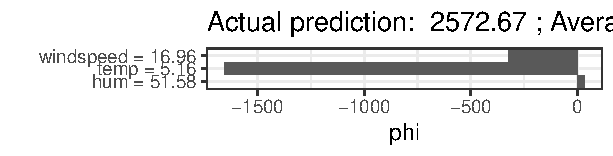
\includegraphics[width=0.9\columnwidth]{figure/shapley2shap.pdf}
\end{figure}
\end{column}
\end{columns}




\end{vbframe}

\begin{vbframe}{SHAP Definition}
\textbf{Aim}: 
Find an additive combination that explains the prediction of an instance $\xv$ by computing the contribution of each feature to the prediction.
\vspace{1cm}
\begin{exampleblock}{}
\[
g\left(\tikzmark{z} z^{\prime}\right)=
\tikzmark{ph0}\phi_{0}+\sum_{j=1}^{M}
\tikzmark{phj} \phi_{j} z_{j}^{\prime}
\]
\begin{tikzpicture}[
  remember picture,
  overlay,
  expl/.style={draw=blue,fill=white,rounded corners,text width=3cm},
  arrow/.style={blue,ultra thick,->,>=latex}
]
\node<1-3>[expl] 
  (zex) 
  at (2,1.5cm)
  {$z^{\prime}$:\textbf{Coalition} \\ simplified features};
\node<2-3>[expl] 
  (ph0ex) 
  at (5,-.5cm)
  {$\phi_0$: \textbf{Null Output} \\ Average Model Baseline};
\node<3>[expl] 
  (phjex) 
  at (12,0cm)
  {$\phi_j$: \textbf{Attribution} \\ How much does feature $j$ change the output};

\draw<1-4>[arrow]
  (zex.east) to[out=180,in=90] ([xshift= 1ex, yshift=1.5ex]{pic cs:z});  
\draw<2-3>[arrow]
  (ph0ex.east) to[out=180,in=270] ([xshift= 1ex, yshift=-0.5ex]{pic cs:ph0});  
\draw<3>[arrow]
  (phjex.west) to[out=90,in=270] ([xshift= 1ex, yshift=-0.5ex]{pic cs:phj});
 \node<4>[expl] 
  (zex)  
  at (2,1cm)
  {$g(z^{\prime})$:\textbf{Marginal Contribution} \\ Contribution of coalition $z^{\prime}$ to the prediction};
\node<4>[expl] 
  (phjsh) 
  at (11,1.5cm)
  {$\phi_j$: \textbf{Shapley Values}};
\draw<4>[arrow]
  (phjsh.west) to[out=90,in=90] ([xshift= 1ex, yshift=1ex]{pic cs:phj}); 
\draw<4> [
    thick,
    decoration={
        brace,
        mirror,
        raise=0.5cm
    },
    decorate
] (7,0.7) -- (9.5,0.7)
node[pos=0.5,below=15pt,black]{\textbf{Additive Feature Attribution}};
\end{tikzpicture}
\end{exampleblock}
\begin{onlyenv}<4>
\vspace{1cm}
\textbf{Problem}\\
How do we estimate the Shapley values $\phi_j$?
\end{onlyenv}

\end{vbframe}



%\begin{vbframe}{Example}

%Given the following example from the bike sharing data set

%\begin{table}[h]
%\centering
%\begin{tabular}{l rrrrr || r}
%  \hline
%  && temperature & humidity & windspeed & year & prediction\\ 
%  \hline
% example $x_{ex}$ && 24.27 & 58.5 & 13.96 & 2011 & 6825 \\ 
% \hline
%\end{tabular}
%\end{table}

%we are searching for Shapley values such that
%\begin{equation}
%\begin{array}{lllllcr}
%\phi_0 &+ \phi_{temp} &+ \phi_{hum} &+ \phi_{windspeed} &+ \phi_{yr} & = &\hat{y} \\
%4469 &+ 1809 &+ 450 &+ 241 &- 144 & = & 6825
%\end{array}
%\end{equation}

%\begin{figure}
 %   \centering
 %   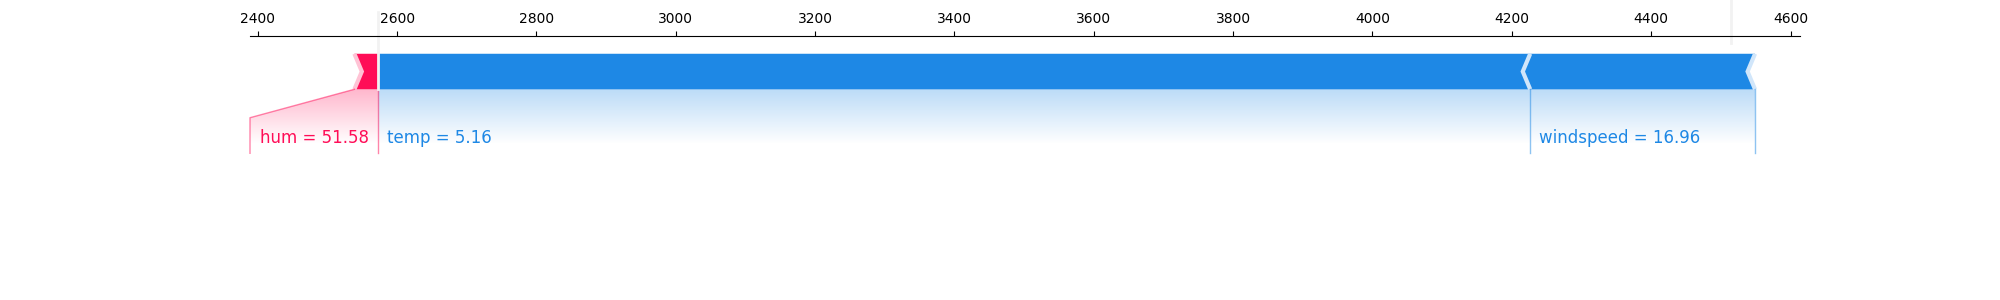
\includegraphics[width=\columnwidth]{slides/shapley/figure_man/exSHAP.png}
%\end{figure}
%\end{vbframe}

\begin{vbframe}{Kernel SHAP - In 5 Steps}

\textbf{Definition:} A kernel-based, model-agnostic method to compute SHAP values via local surrogate models\\
\vspace{1cm}
\begin{enumerate}
    \item Sample Coalitions 
    %\begin{onlyenv}<1>
   % $$z_{k}^{\prime} \in\{0,1\}^{M}, \quad k \in\{1, \ldots, K\}$$
    %\end{onlyenv}
    
    \item Transfer Coalitions into feature space \& get predictions by applying ML model
    
 %   \begin{onlyenv}<2>
  %  $$\hat{f}: \hat{f}\left(h_{x}\left(z_{k}^{\prime}\right)\right)$$
   % \end{onlyenv}
    
    \item Compute weights through Kernel
 %   \begin{onlyenv}<3>
 %   $$\pi_{x}\left(z^{\prime}\right)=\frac{(M-1)}{\left(\begin{array}{c} M \\\left|z^{\prime}\right|\end{array}\right)\left|z^{\prime}\right|\left(M-\left|z^{\prime}\right|\right)}$$
 %   \end{onlyenv}
    
    \item Fit a weighted linear model 
  %  \begin{onlyenv}<4>
  %  $$L\left(\hat{f}, g, \pi_{x}\right)=\sum_{z^{\prime} \in Z}\left[\hat{f}\left(h_{x}\left(z^{\prime}\right)\right)-g\left(z^{\prime}\right)\right]^{2} \pi_{x}\left(z^{\prime}\right)$$
  %  \end{onlyenv}

    \item Return shapley values
%    \begin{onlyenv}<5>
%    $$(\phi_1, \ldots, \phi_M)$$
%    \end{onlyenv}
    
    
\end{enumerate}

\end{vbframe}

\begin{vbframe}{Kernel SHAP - In 5 Steps}


\textbf{Step 1: Sample coalitions}
\begin{itemize}
    \item Sample K coalitions of the simplified feature space
    $$z_{k}^{\prime} \in\{0,1\}^{p}, \quad k \in\{1, \ldots, K\}$$
    \item for our example we receive in total 8 coalitions
\end{itemize}

\begin{table}[]
    \centering
     \begin{tabular}{l |cccc}
  Coalition &  hum & temp & ws \\
  \hline 
  $z^{\prime}_{0}$ & 0 & 0 & 0  \\
   $z^{\prime}_{hum}$ & 1 & 0 & 0  \\
    $z^{\prime}_{temp}$ & 0 & 1 & 0  \\
     $z^{\prime}_{ws}$ & 0 & 0 & 1  \\
     $z^{\prime}_{hum, temp}$ & 1 & 1 & 0  \\
     $z^{\prime}_{temp, ws}$ & 0 & 1 & 1  \\
     $z^{\prime}_{hum, ws}$ & 1 & 0 & 1  \\
  $z^{\prime}_{hum, temp, ws}$ & 1 & 1 & 1  \\
  
 
  \end{tabular}
\end{table}

\end{vbframe}

\begin{vbframe}{Kernel SHAP - In 5 Steps}


\textbf{Step 2: Transfer Coalitions into feature space \& get predictions by applying ML model}
\begin{itemize}
   % \item $$\hat{f}: \hat{f}\left(h_{x}\left(z_{k}^{\prime}\right)\right)$$
    \item We define a coalition $z^{\prime}$, by describing a function 
$h\left(z^{\prime}\right)=x^\prime \text { where } h:\{0,1\}^{p} \rightarrow \mathbb{R}^{p}$
 \item $h(\cdot)$ maps 1’s to the corresponding value from the instance x that we want to explain
    \item it maps 0’s to the values of another instance that we sample from the data
\end{itemize}


\begin{tikzpicture}
\centering


\node (tab1) {%
       \begin{tabular}{l |cccc}
  Coalition &  hum & temp & ws \\
  \hline 
  $z^{\prime}_{0}$ & $\varnothing$ & $\varnothing$ &$\varnothing$  \\
   $z^{\prime}_{hum}$ & 51.6 & $\varnothing$ & $\varnothing$  \\
    $z^{\prime}_{temp}$ & $\varnothing$ & 5.1 & $\varnothing$  \\
     $z^{\prime}_{ws}$ & $\varnothing$ & $\varnothing$ & 17.0  \\
     $z^{\prime}_{hum, temp}$ & 51.6 & 5.1 & $\varnothing$  \\
     $z^{\prime}_{temp, ws}$ &$\varnothing$ & 5.1 & 17.0  \\
     $z^{\prime}_{hum, ws}$ & 51.6 & $\varnothing$ & 17.0  \\
  $z^{\prime}_{hum, temp, ws}$ &51.6 & 5.1 & 17.0   \\
  
 
  \end{tabular}};

\node [left=of tab1] (tab2) {%
     \begin{tabular}{l |cccc}
  Coalition &  hum & temp & ws \\
  \hline 
  $z^{\prime}_{0}$ & 0 & 0 & 0  \\
   $z^{\prime}_{hum}$ & 1 & 0 & 0  \\
    $z^{\prime}_{temp}$ & 0 & 1 & 0  \\
     $z^{\prime}_{ws}$ & 0 & 0 & 1  \\
     $z^{\prime}_{hum, temp}$ & 1 & 1 & 0  \\
     $z^{\prime}_{temp, ws}$ & 0 & 1 & 1  \\
     $z^{\prime}_{hum, ws}$ & 1 & 0 & 1  \\
  $z^{\prime}_{hum, temp, ws}$ & 1 & 1 & 1  \\
  
 
  \end{tabular}};
\draw[->]
(tab2.north) to[out=30,in=150] node[below]{$h(\cdot)$} (tab1.north) ;
\end{tikzpicture}


   




\end{vbframe}


\begin{vbframe}{Kernel SHAP - In 5 Steps}


\textbf{Step 2: Transfer Coalitions into feature space \& get predictions by applying ML model}
\begin{itemize}
   % \item $$\hat{f}: \hat{f}\left(h_{x}\left(z_{k}^{\prime}\right)\right)$$
   \item absent feature values are replaced by feature values of a \color{orange}{random instance} \color{black} of the dataset (permuted) $\leadsto$ permute feature values several times
   \item predict with ML model on this dataset $\hat{f}: \hat{f}\left(h_{x}\left(z_{k}^{\prime}\right)\right)$
\end{itemize}


\begin{tikzpicture}
\centering


\node (tab1) {%
       \begin{tabular}{l |ccc | c}
  Coalition &  hum & temp & ws & $\hat{f}\left(h_{x}\left(z_{k}^{\prime}\right)\right)$\\
  \hline 
  $x^{\prime}_{0}$ & \color{orange}{64.3} & \color{orange}{28.0} & \color{orange}{14.5} & 6211 \\
   $x^{\prime}_{hum}$ & 51.6 & \color{orange}{28.0} & \color{orange}{14.5} & 5586  \\
    $x^{\prime}_{temp}$ & \color{orange}{64.3} & 5.1 & \color{orange}{14.5}  & 3295\\
     $x^{\prime}_{ws}$ & \color{orange}{64.3} & \color{orange}{28.0} & 17.0 &5762 \\
     $x^{\prime}_{hum, temp}$ & 51.6 & 5.1 & \color{orange}{14.5}  & 2616\\
     $x^{\prime}_{temp, ws}$ &\color{orange}{64.3} & 5.1 & 17.0  & 2900\\
     $x^{\prime}_{hum, ws}$ & 51.6 & \color{orange}{28.0} & 17.0 & 5411 \\
  $x^{\prime}_{hum, temp, ws}$ &51.6 & 5.1 & 17.0 & 2573  \\
  
 
  \end{tabular}};

\node [left=of tab1] (tab2) {%
     \begin{tabular}{l |cccc}
  Coalition &  hum & temp & ws \\
  \hline 
  $z^{\prime}_{0}$ & 0 & 0 & 0  \\
   $z^{\prime}_{hum}$ & 1 & 0 & 0  \\
    $z^{\prime}_{temp}$ & 0 & 1 & 0  \\
     $z^{\prime}_{ws}$ & 0 & 0 & 1  \\
     $z^{\prime}_{hum, temp}$ & 1 & 1 & 0  \\
     $z^{\prime}_{temp, ws}$ & 0 & 1 & 1  \\
     $z^{\prime}_{hum, ws}$ & 1 & 0 & 1  \\
  $z^{\prime}_{hum, temp, ws}$ & 1 & 1 & 1  \\
  
 
  \end{tabular}};
\draw[->]
(tab2.north) to[out=30,in=150] node[below]{$h(\cdot)$} (tab1.north) ;
\end{tikzpicture}


   




\end{vbframe}

\begin{vbframe}{Kernel shap - in 5 steps}
\textbf{Step 3: Compute weights through Kernel}\\\medskip
\textbf{Intuition}: We learn most about individual features if we can study their effects in isolation or at maximal interaction:
Small coalitions (few 1’s) and large coalitions (i.e. many 1’s) get the largest weights

\begin{onlyenv}<1>
\begin{figure}
    \centering
    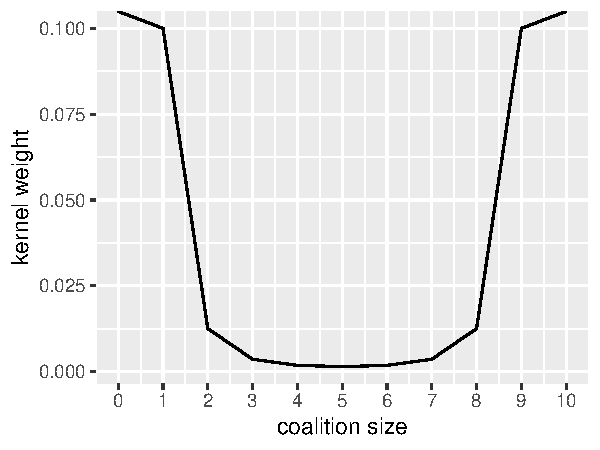
\includegraphics[width=0.5\columnwidth]{slides/shapley/figure_man/kernel-weights.pdf}
\end{figure}
\end{onlyenv}


\begin{onlyenv}<2>
\vspace{1cm}
\begin{exampleblock}{}
\[
\tikzmark{pi}\pi_{x}\left(z^{\prime}\right)=\frac{(
\tikzmark{M}p-1)}{\left(\begin{array}{c} p \\\left|z^{\prime}\right|\end{array}\right)\left|
\tikzmark{z}z^{\prime}\right|\left(p-\left|z^{\prime}\right|\right)}
\]
\begin{tikzpicture}[
  remember picture,
  overlay,
  expl/.style={draw=blue,fill=white,rounded corners,text width=3cm},
  arrow/.style={blue,ultra thick,->,>=latex}
]
\node[expl] 
  (piex) 
  at (4,0cm)
  {$\pi_x(z^{\prime})$: kernel weight for coalition $z^{\prime}$};
\node[expl] 
  (Mex) 
  at (13,2cm)
  {p: Number of features in x};
\node[expl] 
  (zex) 
  at (8,-1cm)
  {$\mid z^{\prime}\mid$: coalition size / sum of 1s in $z^{\prime}$};
\draw[arrow]
  (piex.west) to[out=180,in=135] ([xshift= 0.5ex, yshift=2ex]{pic cs:pi}); 
\draw[arrow]
  (Mex.west) to[out=180,in=135] ([xshift= 0.5ex, yshift=2ex]{pic cs:M}); 
\draw[arrow]
  (zex.north) to[out=180,in=250] ([xshift= 0.5ex, yshift=-1ex]{pic cs:z}); 
\end{tikzpicture}
\end{exampleblock}
\end{onlyenv}


%\begin{onlyenv}<3>

%$$\pi_{x}\left(z^{\prime}\right)=\frac{(M-1)}{\left(\begin{array}{c} M \\\left|z^{\prime}\right|\end{array}\right)\left|z^{\prime}\right|\left(M-\left|z^{\prime}\right|\right)}$$

%\begin{itemize}
%    \item If a coalition consists of a single feature, we can learn about this feature’s isolated main effect on the prediction
%    \item If a coalition consists of all but one feature, we can learn about this feature’s total effect (main effect plus feature interactions)
%    \item If a coalition consists of half the features, we learn little about an individual feature’s contribution, as there are many possible coalitions with half of the features
%\end{itemize}
%\end{onlyenv}

%\begin{onlyenv}<4>
%\vspace{1cm}
%\textbf{Limited Budget $K$}: Can we be a bit smarter about the sampling of coalitions, than just randomly drawing?
%\begin{itemize}
%    \item The smallest and largest coalitions take up most of the weight\\ We get better Shapley value estimates by using some of the sampling budget K to include these high-weight coalitions
%    \item We start with all possible coalitions with 1 and M-1 features, which makes 2 times M coalitions in total\\ When we have enough budget left (current budget is K - 2M), we can include coalitions with 2 features and with M-2 features and so on.
%    \item From the remaining coalition sizes, we sample with readjusted weights
%\end{itemize}
%\end{onlyenv}
  
\end{vbframe}


\begin{vbframe}{Kernel shap - in 5 steps}
\textbf{Step 3: Compute weights through Kernel}\\\medskip
\textbf{Purpose}: to include this knowledge in the local surrogate model (linear regression), we calculate weights for each coalition which are the instances of the linear regression
\only<1>{    $$\pi_{x}\left(z^{\prime}\right)=\frac{(p-1)}{\left(\begin{array}{c} p \\|z^{\prime}|\end{array}\right)|z^{\prime}|(p-|z^{\prime}|)} \leadsto \pi_x\left(z^{\prime} = (1,0,0)\right)=\frac{(3-1)}{\left(\begin{array}{c} 3 \\1\end{array}\right)1\left(3-1\right)} = \frac{1}{3}$$
}

\begin{table}[]
    \centering
        \begin{tabular}{l |ccc|c}
  Coalition &  hum & temp & ws & weight \\
  \hline 
  $z^{\prime}_{0}$ & 0 & 0 & 0 & $\infty$ \\
   $z^{\prime}_{hum}$ & 1 & 0 & 0 & 0.33 \\
    $z^{\prime}_{temp}$ & 0 & 1 & 0 & 0.33 \\
     $z^{\prime}_{ws}$ & 0 & 0 & 1 & 0.33 \\
     $z^{\prime}_{hum, temp}$ & 1 & 1 & 0 & 0.33 \\
     $z^{\prime}_{temp, ws}$ & 0 & 1 & 1 &0.33 \\
     $z^{\prime}_{hum, ws}$ & 1 & 0 & 1 & 0.33 \\
  $z^{\prime}_{hum, temp, ws}$ & 1 & 1 & 1 & $\infty$ \\
  
 
  \end{tabular}
\end{table}
\medskip
\only<2>{
$\leadsto$ weights for empty and full set are infinity and not used as instances for the linear regression\\ $\leadsto$ instead constraints are used such that properties (local accuracy and missingness) are satisfied
}

  
\end{vbframe}

%\begin{vbframe}{Coalition Mapping}
%We define a coalition $z^{\prime}$, by describing a function 

%$$
%h\left(z^{\prime}\right)=z \text { where } h:\{0,1\}^{M} \rightarrow \mathbb{R}^{p}
%$$


%\begin{onlyenv}<1>
%\vspace{1cm}
%\begin{itemize}
%    \item Coalition $z^{\prime} \in \{0, 1\}^M$ is the  vector, indicating if feature $j$ contributes to the prediction 
%    \item $h(\cdot)$ represent a function that maps 1’s to the corresponding value from the instance x that we want to explain: $h(\cdot)$ connects our coalition vector to the underlying data 
%\end{itemize}
%\end{onlyenv}

%\begin{onlyenv}<2->
%\begin{tikzpicture}
%\centering

%\node<2> (tab1) {%
%  \begin{tabular}{l |cccc}
%  Instance & temp & hum & ws & yr\\
%  \hline 
%  $x_{ex}$ & 24.7 & 58.5 & 13.96 & 2011\\
 % \\
 % \\
  %\end{tabular}};
%\node<3-> (tab1) {%
%  \begin{tabular}{l |cccc}
%  Instance & temp & hum & ws & yr\\
%  \hline 
%  $x_{ex}$ & 24.7 & 58.5 & 13.96 & 2011\\
%  $z_{temp, yr}$ & 24.7 & $\varnothing$ & $\varnothing$ & 2011\\
%  $z_{yr}$ & $\varnothing$ & $\varnothing$ & $\varnothing$ & 2011\\
%  \end{tabular}};
%\node<2> [left=of tab1] (tab2) {%
%  \begin{tabular}{l |cccc}
%  Coalition & temp & hum & ws & yr\\
%  \hline 
%  $x^{\prime}$ & 1 & 1 & 1 & 1 \\
%  \\
%  \\
%  \end{tabular}};
%\node<3-> [left=of tab1] (tab2) {%
%  \begin{tabular}{l |cccc}
%  Coalition & temp & hum & ws & yr\\
%  \hline 
%  $x^{\prime}$ & 1 & 1 & 1 & 1 \\
%  $z^{\prime}_{temp, yr}$ & 1 & 0 & 0 %& 1 \\
%  $z^{\prime}_{yr}$ & 0 & 0 & 0 & 1 %\\
%  \end{tabular}};
%\draw<2->[->]
%(tab2.north) to[out=30,in=150] node[below]{$h(\cdot)$} (tab1.north) ;
%\end{tikzpicture}
%\end{onlyenv}
%\begin{onlyenv}<3->
%\begin{itemize}
%    \item $h(\cdot)$ maps 1’s to the %corresponding value from the instance x that we want to explain
%    \item<4> it maps 0’s to the values of another instance that we sample from the data
%    \item<4>  we equate “feature value is absent” with “feature value is replaced by random feature value from data”
%\end{itemize}
%\end{onlyenv}
%\end{vbframe}


\begin{vbframe}{Kernel shap - in 5 steps}
\textbf{Step 4: Fit a weighted linear model}\\\medskip
\textbf{Aim}: Estimate a weighted linear model with Shapley values being the coefficients $\phi_j$
\[
g\left(z^{\prime}\right)=
\phi_{0}+\sum_{j=1}^{p}
 \phi_{j} z_{j}^{\prime}
\]
\only<1>{
and minimize by WLS using the weights of step 3
    $$L\left(\hat{f}, g, \pi_{x}\right)=\sum_{z^{\prime} \in Z}\left[\hat{f}\left(h_{x}\left(z^{\prime}\right)\right)-g\left(z^{\prime}\right)\right]^{2} \pi_{x}\left(z^{\prime}\right)$$

with $\phi_0 = E(\fh)$ and $\phi_p = \fh(x) - \sum_{j=0}^{p-1} \phi_j$ we receive a $p-1$ dimensional linear regression problem
}

\only<2>{
\begin{table}[]
    \centering
        \begin{tabular}{l |ccc|c|c}
  Coalition &  hum & temp & ws & weight & $\fh$\\
  \hline 
   $z^{\prime}_{hum}$ & 1 & 0 & 0 & 0.33 & 4635\\
    $z^{\prime}_{temp}$ & 0 & 1 & 0 & 0.33 & 3087\\
     $z^{\prime}_{ws}$ & 0 & 0 & 1 & 0.33 & 4359\\
     $z^{\prime}_{hum, temp}$ & 1 & 1 & 0 & 0.33 & 3060\\
     $z^{\prime}_{temp, ws}$ & 0 & 1 & 1 &0.33 & 2623\\
     $z^{\prime}_{hum, ws}$ & 1 & 0 & 1 & 0.33 & 4450\\
  
 
  \end{tabular}
\end{table}
}

  
\end{vbframe}

\begin{vbframe}{Marginal Contribution}

\begin{itemize}
    \begin{onlyenv}<1>
    \item Consider coalition $z^{\prime}$ as indicator function for our shapley values $\phi$
    \end{onlyenv}
    \begin{onlyenv}<2>
    \item This connects the coalition vector $z^{\prime}$ to the respective marginal contribution
    \end{onlyenv}
    \begin{onlyenv}<3>
    \item To estimate the marginal contribution, we can transfer the coalition to the data space by $h(z^{\prime})$
    \end{onlyenv}
    \begin{onlyenv}<4->
    \item $\fh(h(z^{\prime}))$ connects the coalitions directly to the marginal distribution.
    \end{onlyenv}
\end{itemize}

\vspace{1cm}

\begin{tikzpicture}
\centering

\node<1-2> (tab1) {%
  \begin{tabular}{l |cccc}
  Coalition & temp & hum & ws & yr\\
  \hline 
  $x^{\prime}$ & 1 & 1 & 1 & 1 \\
  $z^{\prime}_{temp, yr}$ & 1 & 0 & 0 & 1 \\
  $z^{\prime}_{yr}$ & 0 & 0 & 0 & 1 \\
  \end{tabular}};
\node<2-> [right=of tab1] (tab2) {%
\begin{tabular}{l | cccc}
  & temp & hum & ws & yr\\
  \hline 
  $g(x^{\prime})$ & $\phi_{temp}$ + & $\phi_{hum}$ + & $\phi_{ws}$ + & $\phi_{yr}$ \\
  $g(z^{\prime}_{temp, yr})$ & $\phi_{temp}$ + &  &  & $\phi_{yr}$\\
   $g(z^{\prime}_{yr})$ & &  &  & $\phi_{yr}$ \\
  \end{tabular}};
\node<3-> [left=of tab2] (tab) {%
  \begin{tabular}{l |cccc}
  Instance & temp & hum & ws & yr\\
  \hline 
  $x_{ex}$ & 24.7 & 58.5 & 13.96 & 2011\\
  $z_{temp, yr}$ & 24.7 & $\varnothing$ & $\varnothing$ & 2011\\
  $z_{yr}$ & $\varnothing$ & $\varnothing$ & $\varnothing$ & 2011\\
  \end{tabular}};
\draw<2>[->]
(tab1.south) to[out=320,in=200] node[above]{$\sum \mathbb{I}_{[z^{\prime}_i == 1]} \phi_i$} (tab2.south) ;
\draw<3->[->]
(tab2.south) to[out=200,in=330] node[above]{$\fh(h(z^{\prime}))$} (tab1.south) ;
\end{tikzpicture}

\begin{onlyenv}<4>
\begin{equation}
\begin{array}{lllc}
  
  g(x^{\prime}) &= \phi_{temp} + \phi_{hum} + \phi_{ws} + &\phi_{yr} &= 6825\\
  g(z^{\prime}_{temp, yr}) &= \phi_{temp} + &\phi_{yr} &= 6134\\
   g(z^{\prime}_{yr}) &= &\phi_{yr} &= 4325\\
\end{array}
\end{equation}
\end{onlyenv}

\begin{onlyenv}<5>
\vspace{0.5cm}

\textbf{Notice:}\\ We created a coalition data set $Z^{\prime}$ here by sampling multiple coalitions from instance $\xv$ that is evaluable with the prediction function $\fh$
\end{onlyenv}

\end{vbframe}





\begin{vbframe}{Properties}

\textbf{Local Accuracy}
$$
f(x)=g\left(x^{\prime}\right)=\phi_{0}+\sum_{j=1}^{M} \phi_{j} x_{i}^{\prime}
$$
\begin{onlyenv}<1>
\textbf{Intution:} If the coalition includes all features ($x^{\prime}  \in \{1\}^M $), the attributions $\phi_j$ should sum up with the base line $\phi_0$ to the original model output for observation $f(\xv)$ \\
Local Accuracy corresponds to the \textbf{Axiom of Efficiency} in Shapley Game Theory 

\end{onlyenv}

\begin{onlyenv}<2->
\textbf{Missingness}
$$
x_{i}^{\prime}=0 \Longrightarrow \phi_{i}=0
$$
\end{onlyenv}

\begin{onlyenv}<2>
\textbf{Intution:}  A missing feature gets an attribution of zero
\end{onlyenv}

\begin{onlyenv}<3->
\textbf{Consistency} \\
\end{onlyenv}
\begin{onlyenv}<3>
$f_{x}\left(z^{\prime}\right)=f\left(h_{x}\left(z^{\prime}\right)\right) \text { and } z^{\prime}_{\backslash  i} \text{ denote setting } z_{i}^{\prime}=0$ . For any two
models $f$ and $f^{\prime}$, if
$$
f_{x}^{\prime}\left(z^{\prime}\right)-f_{x}^{\prime}\left(z^{\prime}_{\backslash i}\right) \geq f_{x}\left(z^{\prime}\right)-f_{x}\left(z^{\prime}_{\backslash i}\right)
$$
for all inputs $z^{\prime} \in \{0, 1\}^M$, then
$$
\phi_{i}\left(f^{\prime}, x\right) \geq \phi_{i}(f, x)
$$
\end{onlyenv}

\begin{onlyenv}<4->
$$
f_{x}^{\prime}\left(z^{\prime}\right)-f_{x}^{\prime}\left(z^{\prime}_{\backslash i}\right) \geq f_{x}\left(z^{\prime}\right)-f_{x}\left(z^{\prime} _{\backslash i}\right) \Longrightarrow \phi_{i}\left(f^{\prime}, x\right) \geq \phi_{i}(f, x)
$$

\textbf{Intution:} If a model changes so that the marginal contribution of a feature value increases or stays the same, the Shapley value also increases or stays the same\\ 
From Consistency the Shapley \textbf{Axioms of Linearity, Dummy and Symmetry} follow
\end{onlyenv}


\end{vbframe}

\begin{vbframe}{Tree SHAP}

TreeSHAP is a fast model specific exact calculation of Shapley values for tree based models

\begin{onlyenv}<1-3>
\vspace{0.5cm}
Consider following Tree:

\textbf{Cases}
Consider the following cases of feature subset S

\begin{itemize}
    \begin{onlyenv}<1>
    \item  S is the set of all features – 
    the prediction from the node in which the instance x falls is be the expected prediction.
    \end{onlyenv}
    \begin{onlyenv}<2>
    \item S is empty -
    use the weighted average of predictions of all terminal nodes in the decision tree. \\
     
    \end{onlyenv}
    \begin{onlyenv}<3>
    \item S contains some, but not all, features -
    ignore predictions of unreachable nodes \& average the predictions item from the remaining terminal nodes weighted by  sizes
    \end{onlyenv}
\end{itemize}

Given instance $x_{ey}$ and the displayed tree
\begin{table}
\begin{columns}[T]
\begin{column}{0.3\textwidth}
\centering
\begin{tabular}{l |rrr}
  \hline
  & temp & year & $\fh$\\ 
  \hline
 $x_{ex}$ & 24.27 & 2011 & 6825 \\ 
 \hline
\end{tabular}
\end{column}
\begin{column}{0.7\textwidth}
\begin{tikzpicture}[
    node/.style={%
      draw=blue,
      rectangle,
      fill=white,
      rounded corners
    },
  ]
\centering
    \node [node, label=below:{n=10}] (A) {year $>$ 2011};
    \path (A) ++(7:3.8cm) node [node, label=below:{n=5}] (B) {count = 3200};
    \path (A) ++(-7:3.8cm) node [node, label=below:{n=5}] (C) {temp $>$ 30};
    \path (C) ++(14:3.8cm) node [node, label=below:{n=3}] (D) {count = 6850};
    \path (C) ++(0:3.8cm) node [node, label=below:{n=2}] (E) {count = 5400};
    

    \draw (A) -- (B) node [left,pos=0.5] {no}(A);
    \draw (A) -- (C) node [right,pos=0.5] {yes}(A);
    \draw (C) -- (D) node [left,pos=0.5] {no}(A);
    \draw (C) -- (E) node [right,pos=0.5] {yes}(A);
    
\end{tikzpicture}
\end{column}
\end{columns}
\end{table}

\begin{onlyenv}<1>
$$
S = \varnothing \rightarrow z^{\prime} = (0, 0) \rightarrow \phi_0 = \frac{3200*5 + 6850*3 +5400*2}{10}= 3775
$$
\end{onlyenv}

\begin{onlyenv}<2>
$$
S = \{x_{temp}, x_{year}\} \rightarrow z^{\prime} = (1, 1)  \rightarrow \phi_{year, temp} = 6850
$$
\end{onlyenv}

\begin{onlyenv}<3>
$$
S = \{x_{temp}\} \rightarrow z^{\prime} = (0, 1)  \rightarrow \phi_{\cdot, temp} = \frac{3200*5 + 3* 6850}{8} = 3625
$$
\end{onlyenv}
\end{onlyenv}

\begin{onlyenv}<4>
\vspace{1.5cm}
\textbf{Complexity:}
\begin{itemize}
    \item Complexity of exact KernelSHAP: $\mathcal{O}(TLD^2)$
    \item Complexity of TreeSHAP: $\mathcal{O}(TL2M)$
\end{itemize}

T is the number of trees, L is the maximum number of leaves in any tree and D the maximal depth of any tree
\end{onlyenv}


\end{vbframe}

 \begin{vbframe}{Global SHAP}
\textbf{Idea: }
\begin{itemize}
    \item Run SHAP for every instance and thereby get a matrix of Shapley values
    \item The matrix has one row per data instance and one column per feature
    \item We can interpret the model globally by analyzing the Shapley values in this matrix
\end{itemize}
\vspace{2cm}
$$
\Phi =
\begin{bmatrix}
    \phi_{11} & \phi_{12} & \phi_{13} & \dots  & \phi_{1M} \\
    \phi_{21} & \phi_{22} & \phi_{23} & \dots  & \phi_{2M} \\
    \vdots & \vdots & \vdots & \ddots & \vdots \\
    \phi_{n1} & \phi_{n2} & \phi_{n3} & \dots  & \phi_{nM} \\
\end{bmatrix}
$$

 \end{vbframe}

 \begin{vbframe}{Feature Importance}
 
\textbf{Idea:} Average the Shapley values of each feature over all instances. This corresponds to calculating column-wise averages in $\Phi$
$$
I_{j}=\frac{1}{n} \sum_{i=1}^{n}\left|\phi_{j}^{(i)}\right|
$$

\begin{figure}
    \centering
    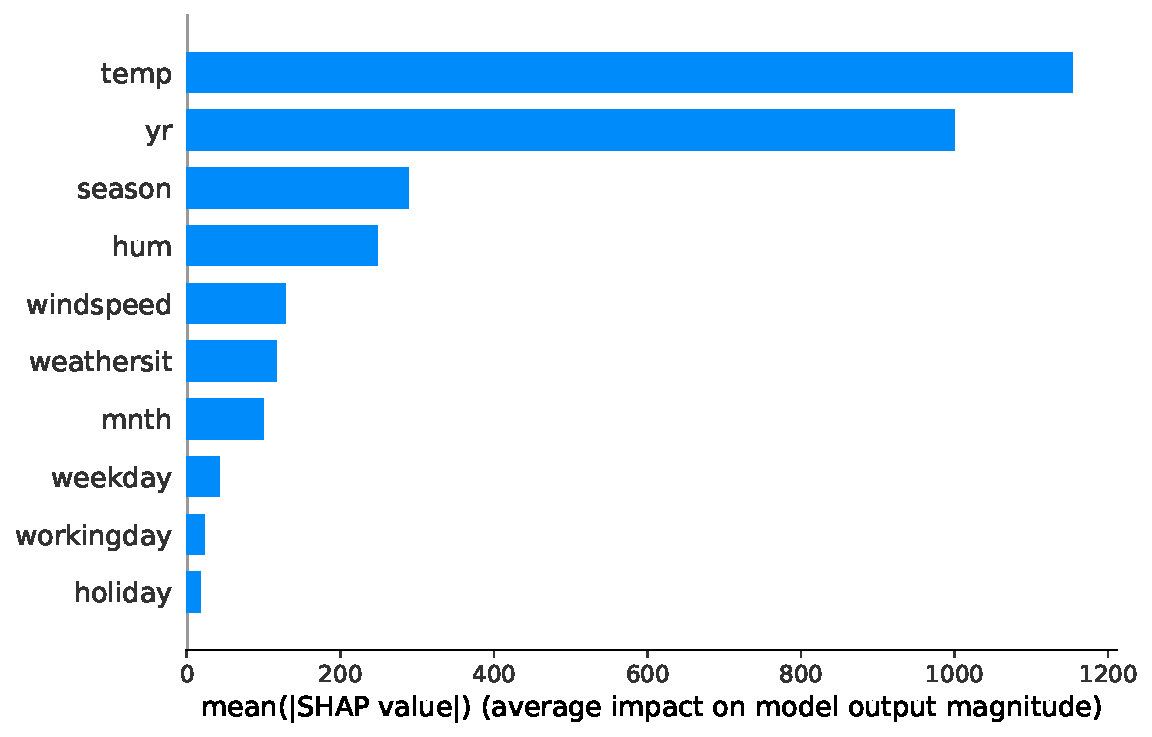
\includegraphics[width=0.5\columnwidth]{slides/shapley/figure_man/global_shap_fi.pdf}
\end{figure}

\end{vbframe}
 
\begin{vbframe}{Summary Plot}

Combines feature importance with feature effects
\begin{itemize}
    \item Each point is a Shapley value for a feature and an instance
    \item The color represents the value of the feature from low to high
    \item Overlapping points are jittered in y-axis direction
\end{itemize}

\begin{figure}
    \centering
    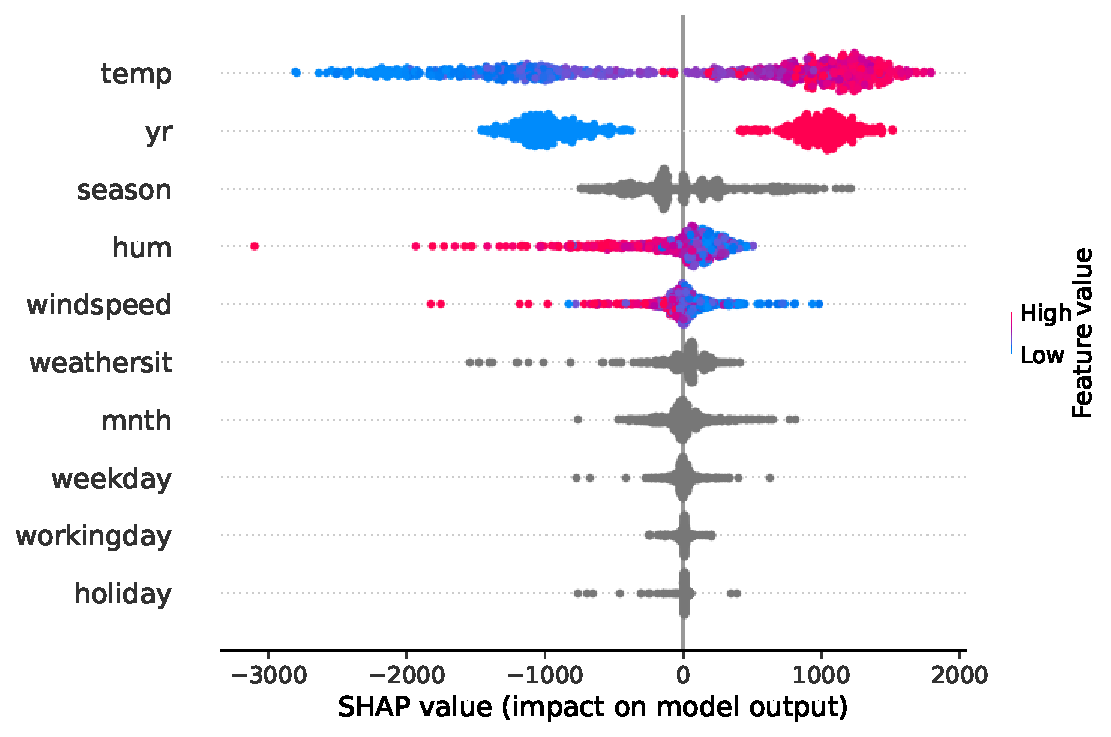
\includegraphics[width=0.5\columnwidth]{slides/shapley/figure_man/global_shap_jitter.pdf}
    
\end{figure}
\end{vbframe} 

\begin{vbframe}{Dependence Plot}
Simply plot a point with the feature value on the x-axis and the corresponding Shapley value on the y-axis

\begin{figure}
    \centering
    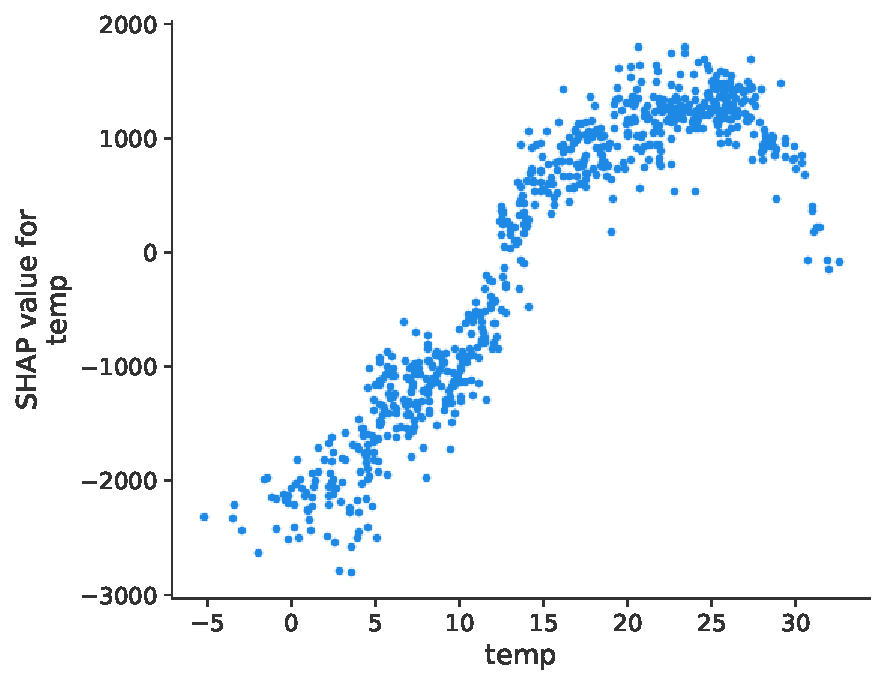
\includegraphics[width=0.5\columnwidth]{slides/shapley/figure_man/global_shap_depend.pdf}
\end{figure}

\end{vbframe}

\begin{vbframe}{Discussion}
\begin{onlyenv}<1>
\textbf{Advantages}

\begin{itemize}
    \item All the advantages of Shapley values
    \begin{itemize}
        \item \textbf{solid theoretical foundation} in game theory
        \item prediction is \textbf{fairly distributed} among the feature values
        \item \textbf{contrastive explanations} that compare the prediction with the average prediction.
    \end{itemize} 
    \item unify the field of interpretable machine learning in the class of additive feature attribution methods
    \item has a fast implementation for tree-based models
    \item various global interpretation methods
\end{itemize}
\end{onlyenv}

\begin{onlyenv}<2>
\textbf{Disadvantages}

\begin{itemize}
    \item KernelSHAP is slow
    \item KernelSHAP ignores feature dependence
    \item TreeSHAP can produce unintuitive feature attributions
    \item disadvantages of Shapley values also apply to SHAP:
    \begin{itemize}
        \item Shapley values can be misinterpreted and access to data is needed to compute them for new data
    \end{itemize}
    \item It is possible to create intentionally misleading interpretations with SHAP, which can hide biases
\end{itemize}


\end{onlyenv}

\end{vbframe}

\endlecture
\end{document}
